

\documentclass[12pt]{extarticle}
\usepackage{summary-intro}









\begin{document}


\sumintro{The Higher Infinite}{Spring 2023}

 

\section{The Ordinals}

\subsection{How We'll Get to the Ordinals}

\[
\text{Ordering} \rightarrow \text{Total Ordering} \rightarrow \text{Well-Ordering} \rightarrow \text{Well-Order Type} \rightarrow \text{Ordinal}
\]


\subsection{Strict Orderings}

Think of $x < y$ as meaning ``$x$ precedes $y$''. We say that $<$ is a \textbf{strict ordering} on set $A$ if and only if for any $a,b,c \in A$:

\begin{description}\label{gloss:ordering}

\item[Asymmetry] If $a<b$ , then not-$(b < a)$. (NOT the same as anti-symmetric!)\label{gloss:asymmetry}

\item[Transitivity] If $a<b$ and $b<c$, then $a<c$.


\end{description}

\subsection{Total Orderings}

A \textbf{total ordering} $<$ on $A$ is an ordering on $A$ such that  for any distinct elements $a, b$ of $A$:


\begin{description}
\item[Totality] $a < b$ \ or \ $b < a$\\[1ex]


\textit{Aside}: Recall that for cardinals we defined a total order $\leq$ that is reflexive, anti-symmetric, and transitive. This $\leq$ is a non-strict total order. Both kinds of orders are transitive, but `non-strict' means reflexive and anti-symmetric, while strict means asymmetric (which entails irreflexive). 

\end{description}


\subsection{Well-Orderings}

A \textbf{well-ordering} $<$ of $A$ is a strict total ordering on $A$ such that:


\begin{description}
\item[Well-Ordering]   Every non-empty subset $S$ of $A$ has a $<$-smallest member. 
\end{description}

\subsection{Well-order types}

The orderings $<_1$ and $<_2$ are of the same type if they are isomorphic.\footnote{Let $<_1$ be an ordering on $A$ and $<_2$ be an ordering on $B$. Then  $<_1$ is \textbf{isomorphic} to $<_2$ if and only if there is a bijection $f$ from $A$ to $B$ such that, for every $x$ and $y$ in $A$, $x<_1y$ if and only if $f(x)<_2f(y)$.
}

%%%%

\subsection{The First Few Ordinals}

\[
\begin{array}{ccc}
\text{ordinal} & \text{name of ordinal} & \text{well-order type represented}\\ \hline
\set{} &0 & \ \\
\set{0} &0'  & |   \\
\set{0,0'} &0''  & | |  \\
\set{0,0',0''} &0''' & | | |  \\
\vdots  & \vdots\\
\set{0,0',0'',0''',\dots} &\omega  & | | |  \dots   \\
\set{0,0',0'',0''',\dots,\omega} &\omega'  & | |  | \dots |  \\
\set{0,0',0'',0''',\dots,\omega, \omega'} &\omega''  & | | | \dots | |  \\
\vdots & \vdots & \vdots \\
\end{array}
\]

\subsection{Constructing the Ordinals}

 \begin{description}
\item[Construction Principle] 
At each stage, we introduce a new ordinal, namely: the set of all ordinals that have been introduced at previous stages.

\end{description}
\begin{description}
\item[Open-Endedness Principle] However many stages have occurred, there is always a ``next'' stage, that is, a first stage after every stage considered so far.\footnote{It is important to interpret the Open-Endedness Principle as entailing that there is no such thing as ``all'' stages---and therefore deliver the result that there is no such thing as ``all'' ordinals.}

\end{description}

\subsection{Ordering the Ordinals}

The ordinals are well-ordered by the following precedence relation:
$$\alpha <_o \beta \leftrightarrow_{\text{\emph{df}}} \alpha \in \beta$$



\subsection{Representing Well-Order Types}


Since every ordinal is a set of ordinals, the elements of an ordinal are always well-ordered by $<_o$. So we may set forth the following:

\begin{description}
\item[Representation Principle] 
Each ordinal represents the well-order type that it itself instantiates under $<_o$.
\end{description}

\subsection{Some Definitions}

\begin{itemize}

\item $\alpha' = \alpha \cup \set{\alpha}$

\item A \textbf{successor ordinal} is an ordinal \(\alpha\) such that \(\alpha = \beta'\) for some \(\beta\).


\item A \textbf{limit ordinal} is an ordinal that is not a successor ordinal.
\end{itemize}


\section{Ordinal Addition}

\textbf{Note}: the intuitive definitions of addition and multiplication will suffice for the problem set! And no need to use exponentiation, tetration, etc. \\[1ex]

\noindent \emph{The intuitive idea:} A well-ordering of type $(\alpha+\beta)$ is the result of starting with a well-ordering of type $\alpha$ and appending a well-ordering of type $\beta$ at the end.

\vspace{2mm}
\noindent
\emph{Formally:}
\vspace{-4mm}
\[
\begin{array}{rclcl}
 \alpha &+ &0 &= &\alpha  \\
 \alpha &+ &\beta' &= &(\alpha + \beta)'\\
 \alpha &+ &\lambda &= & \bigcup \{\alpha + \beta : \beta < \lambda\} \text{ ($\lambda$ a limit ordinal)}
  \end{array}
 \]


\begin{itemize}
\item Ordinal addition is associative: \((\alpha+\beta)+\gamma = \alpha+(\beta+\gamma)\).

\item Ordinal addition is \emph{not} commutative: it is not generally the case that $\alpha + \beta = \beta + \alpha$.
\end{itemize}

\section{Ordinal Multiplication}

\emph{The intuitive idea:} A well-ordering of type $(\alpha\times\beta)$ is the result of starting with a well-ordering of type $\beta$ and replacing each position in the ordering with a well-ordering of type $\alpha$.

\vspace{3mm}

\noindent
\emph{Formally:}
\vspace{-3mm}
\[
\begin{array}{rclcl}
  \alpha &\times &0 &= &0  \\
 \alpha &\times &\beta' &= &(\alpha \times \beta) + \alpha\\
 \alpha &\times &\lambda &= & \bigcup \{\alpha \times \beta : \beta < \lambda\} \text{ ($\lambda$ a limit ordinal)}
 \end{array}
\]

\begin{itemize}
\item Ordinal multiplication is associative: \((\alpha\times\beta)\times\gamma = \alpha\times(\beta\times\gamma)\).

\item Ordinal multiplication is \emph{not} commutative: it is not generally the case that $\alpha \times \beta = \beta \times \alpha$.
\end{itemize}


\section{Some Additional Operations}


\begin{itemize}

\item Exponentiation:
\[
\begin{array}{lcl}
 \alpha^0 &= & 0'  \\
 \alpha^{\beta'} &= &(\alpha^\beta) \times \alpha \\
 \alpha^{\lambda} &= & \bigcup \{\alpha^\beta : \beta < \lambda\} \text{ ($\lambda$ a limit ordinal)}
 \end{array}
\]

\item Tetration:
\[
\begin{array}{lcl}
 ^0\alpha &= & 0'  \\
 ^{\beta'}\alpha &= &(^\beta\alpha)^\alpha \\
 ^{\lambda}\alpha &= & \bigcup \{^\beta\alpha : \beta < \lambda\} \text{ ($\lambda$ a limit ordinal)}
 \end{array}
\]

\item And so forth\dots

\end{itemize}


\begin{landscape}



\section{Some Additional Ordinals}

\[
\begin{array}{ccc}
\text{ordinal} & \text{members} & \text{well-order type represented}\\ \hline
\omega  &\set{0,0',\dots} & | | | \dots   \\ \hline
\omega+0'  &\set{0,0',\dots,\omega} & | | |  \dots  |  \\ \hline
\omega+\omega  &\set{0,0',\dots,\omega, \omega+0',\dots} & | | |  \dots  | | | \dots  \\ \hline
\omega+\omega+\omega  &\set{0,0',\dots,\omega, \omega+0',\dots,\omega+\omega,\omega+\omega+0',\dots} & | | |  \dots  | | | \dots | | | \dots \\ \hline
%
\parbox{11mm}{\vspace{1mm}$\omega\times\omega \\  =  \omega^{0''}$}  &\set{0,\dots,\omega,\dots,\omega+\omega,\dots,\omega+\omega+\omega,\dots \ {\LARGE\dots}} & \underbrace{| | |  \dots  | | | \dots | | | \dots \ {\Large \dots}}_{\omega \text{ times}} \\ \hline
%
(\omega\times\omega)+\omega  &\set{0,\dots,\omega\times\omega,(\omega\times\omega)+0', (\omega\times\omega)+0'', \dots} & \underbrace{| | |  \dots  | | | \dots | | | \dots \ {\Large \dots}}_{\omega \text{ times}} | | | \dots \\ \hline
%
(\omega\times\omega)+\omega+\omega  &\set{0,\dots,\omega\times\omega,(\omega\times\omega)+0', \dots (\omega\times\omega)+\omega, (\omega\times\omega)+\omega + 0' \dots} & \underbrace{| | |  \dots  | | | \dots | | | \dots \ {\Large \dots}}_{\omega \text{ times}} | | | \dots | | | \dots\\ \hline
%
\parbox{31mm}{$(\omega\times\omega)+(\omega\times\omega) \\ \ = \ \  \omega \times \omega \times 0''$} &\set{0,\dots,\omega\times\omega, \dots (\omega\times\omega)+\omega, \dots, (\omega \times \omega) + \omega + \omega \dots \ \dots} & \hspace{-30mm}\parbox{30mm}{\footnotesize $\underbrace{| | |  \dots  | | | \dots | | | \dots \ {\dots}}_{\omega \text{ times}} \ \ \underbrace{| | |  \dots  | | | \dots | | | \dots \ {\dots}}_{\omega \text{ times}}$}\\ \hline
%
\omega\times\omega \times 0'''  & \parbox{110mm}{\vspace{1mm}\scriptsize
$\{0,\dots,\omega\times\omega, \dots (\omega\times\omega)+\omega, \dots, (\omega \times \omega) + \omega + \omega \dots \ \dots \\ (\omega \times \omega) + (\omega \times \omega) \dots (\omega \times \omega) + (\omega \times \omega) + \omega \dots (\omega \times \omega) + (\omega \times \omega) + \omega + \omega \dots \ \dots\}$}
 &  \hspace{-40mm} \parbox{30mm}{\vspace{1mm} \footnotesize $\underbrace{| | |  \dots  | | | \dots \ {\Large \dots}}_{\omega \text{ times}} \ \ \underbrace{| | |  \dots | | | \dots \ {\Large \dots}}_{\omega \text{ times}} \ \ \underbrace{| | |  \dots   | | | \dots \ {\Large \dots}}_{\omega \text{ times}}$}\\\hline
%
\parbox{21mm}{$\omega \times \omega \times \omega \\ \ = \ \ \omega^{0'''}$} &\set{0\dots,\omega\times\omega, \dots \omega\times \omega \times 0'',\dots, \omega\times \omega \times 0''',\dots \ \dots} 
&  \hspace{-20mm} \parbox{30mm}{ \vspace{1mm} \footnotesize $\underbrace{\underbrace{|  | \dots | | \dots \ {\Large \dots}}_{\omega \text{ times}} \ \  \underbrace{| |  \dots  | | \dots \ {\Large \dots}}_{\omega \text{ times}} \ \ \dots}_{\omega \text{ times} }$}\\\hline
%
\omega^\omega &\set{0,\dots,\omega,\dots,\omega \times 0'', \dots,\omega \times 0''', \dots \ \dots} & \text{\scriptsize[see below]}\\ \hline
\end{array}
\]

\vspace{3mm}
{\tiny
$$
\text{\normalsize $\omega^\omega$:}  \quad \quad
| | \dots \
%
\underbrace{| | \dots  | | \dots \ {\Large \dots}}_{\omega \text{ times}} \
%
\underbrace{\underbrace{| |  \dots   | | \dots \ {\Large \dots}}_{\omega \text{ times}} \ \ \underbrace{| |  \dots  | | \dots \ {\Large \dots}}_{\omega \text{ times}} \ \ \dots}_{\omega \text{ times} } \
%%
\underbrace{
\underbrace{\underbrace{| |  \dots  | | \dots \ {\Large \dots}}_{\omega \text{ times}} \ \ \underbrace{| |  \dots  | |  \dots \ {\Large \dots}}_{\omega \text{ times}} \ \ \dots}_{\omega \text{ times} }
%
\underbrace{\underbrace{| |  \dots   | | \dots \ {\Large \dots}}_{\omega \text{ times}} \ \ \underbrace{| |  \dots  | |  \dots \ {\Large \dots}}_{\omega \text{ times}} \ \ \dots}_{\omega \text{ times} }
%
\ \ \dots
}_{\omega \text{ times}}
%%
\text{\large \quad \dots}
$$
}


\end{landscape}

\section{A Visualization\footnote{\ Source: https://commons.wikimedia.org/wiki/File:Omega-exp-omega-labeled.svg.  File made available on Wikimedia under the Creative Commons CC0 1.0 Universal Public Domain Dedication. Pop-up casket (talk); original by User:Fool [CC0].}}

\vspace{-3mm}
\hspace{4mm}
%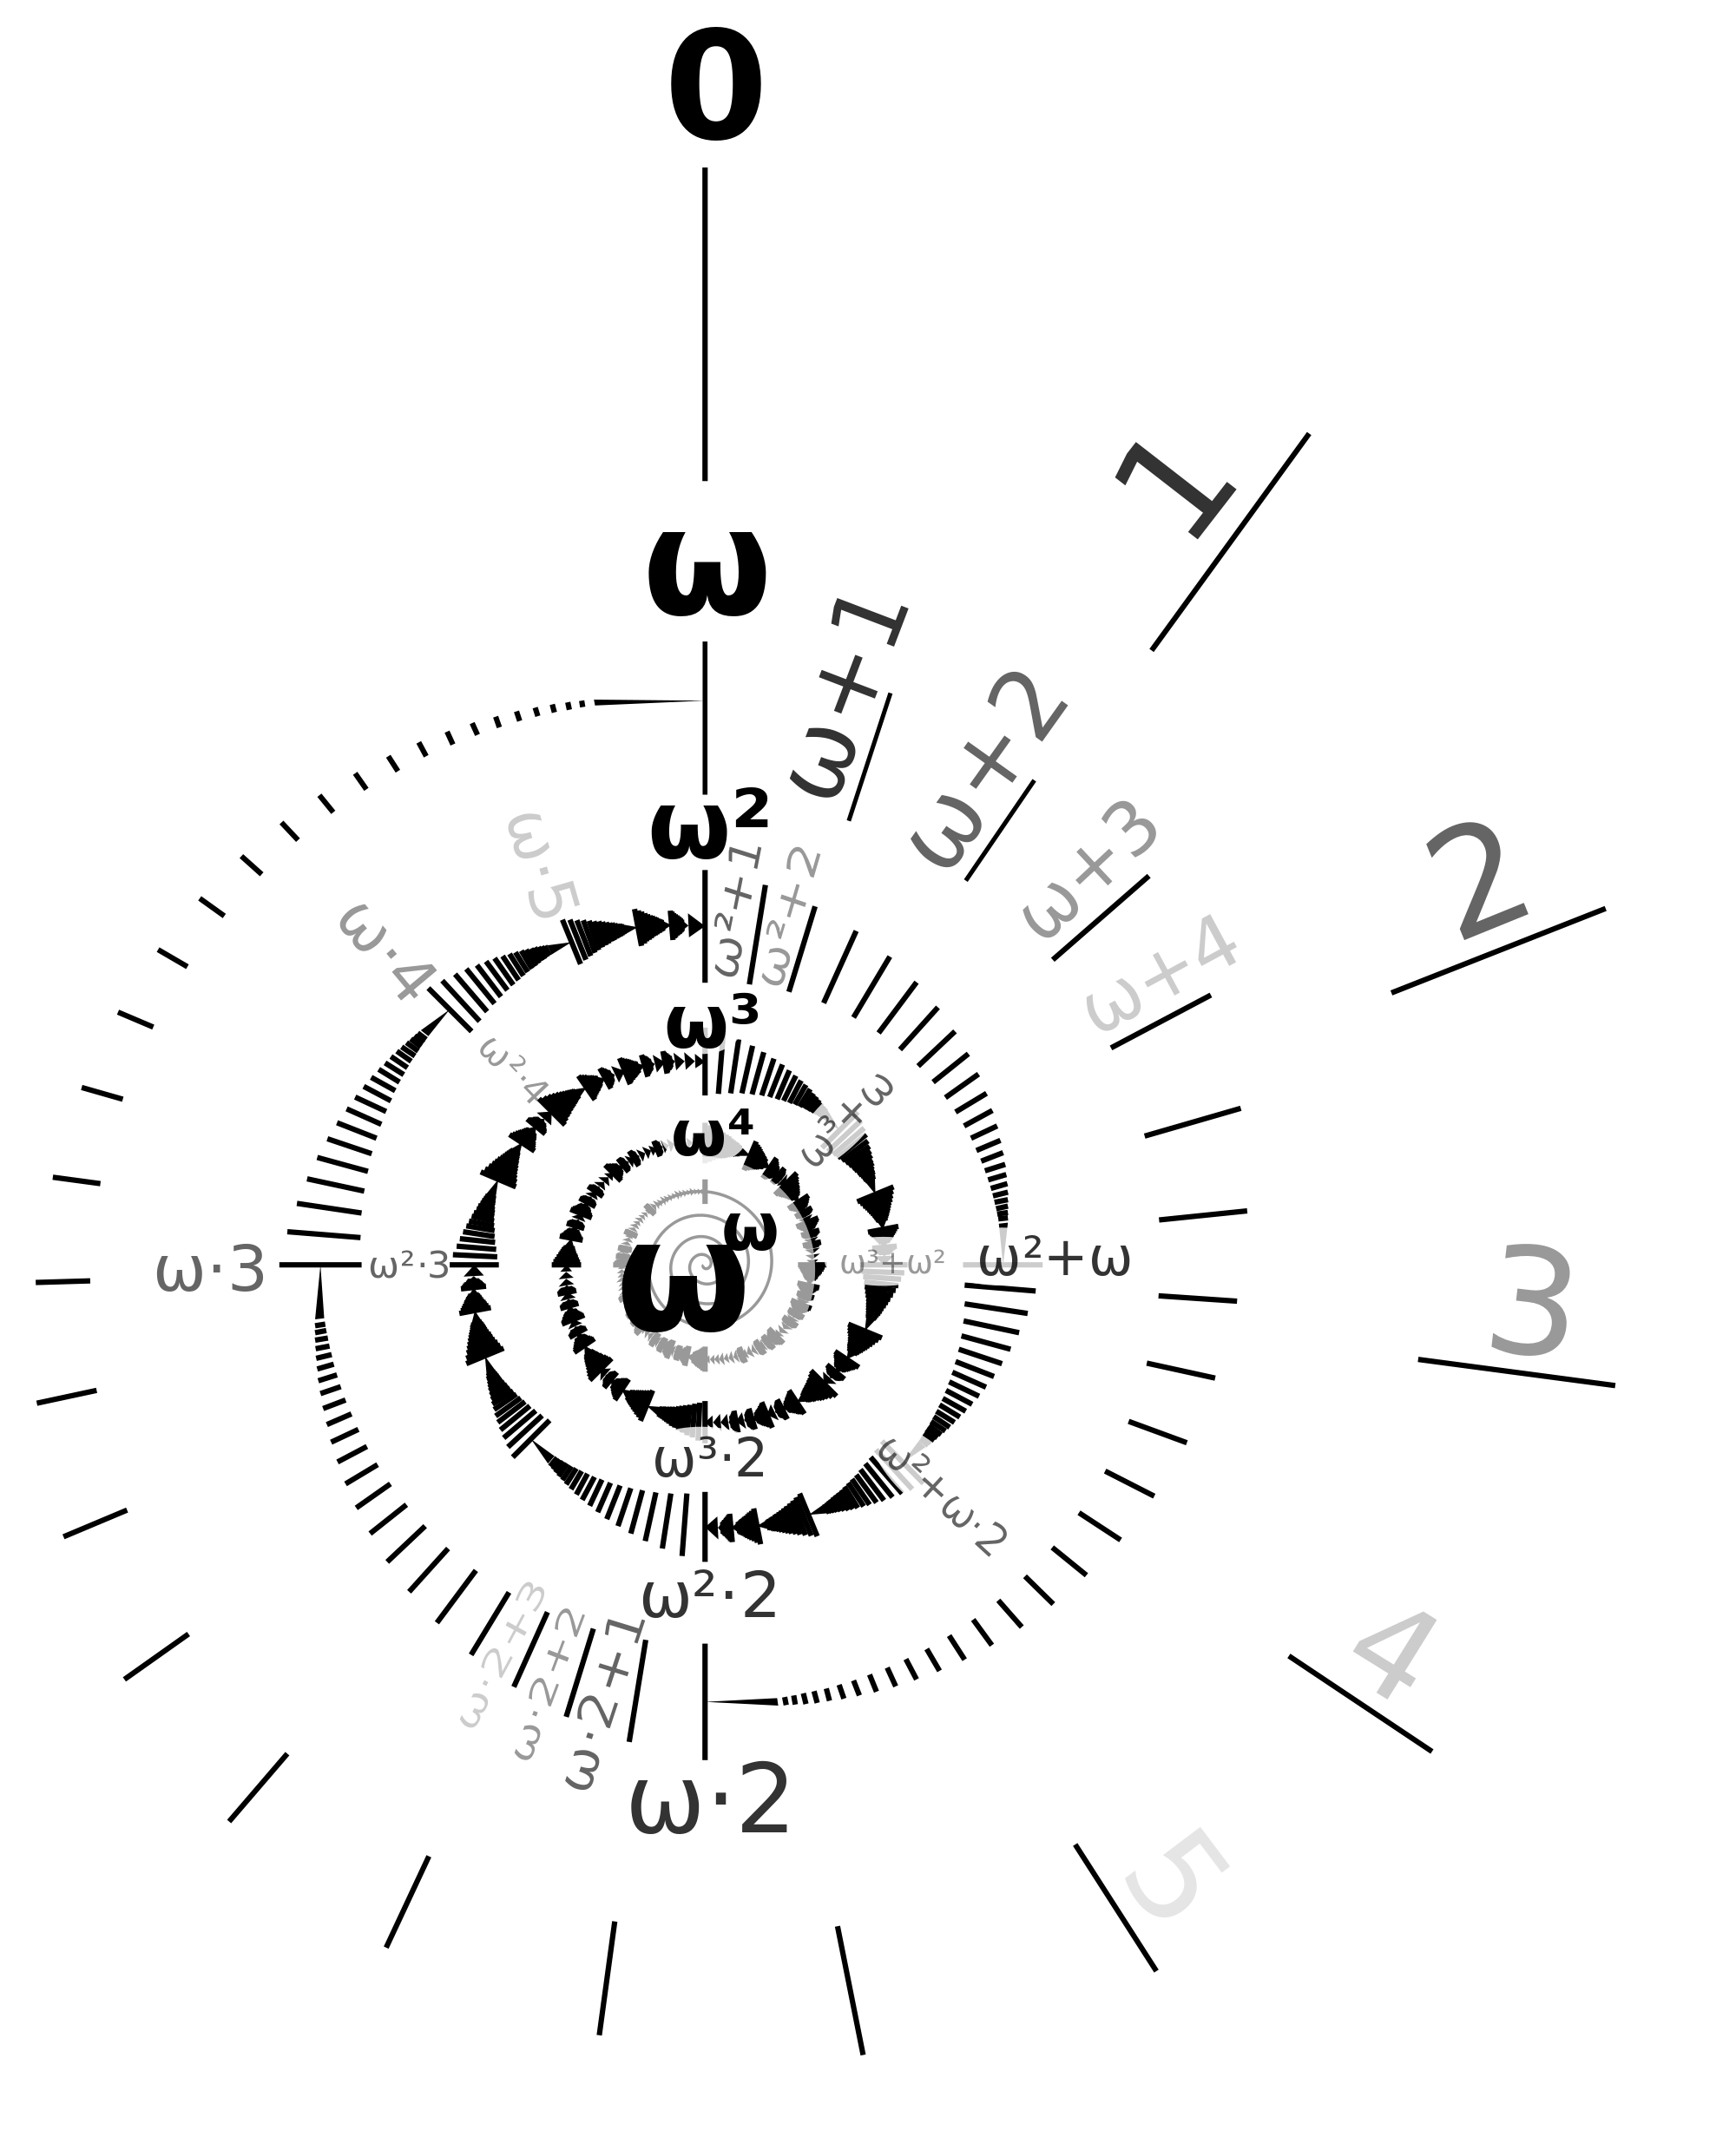
\includegraphics[scale=.19]{Omega.png}
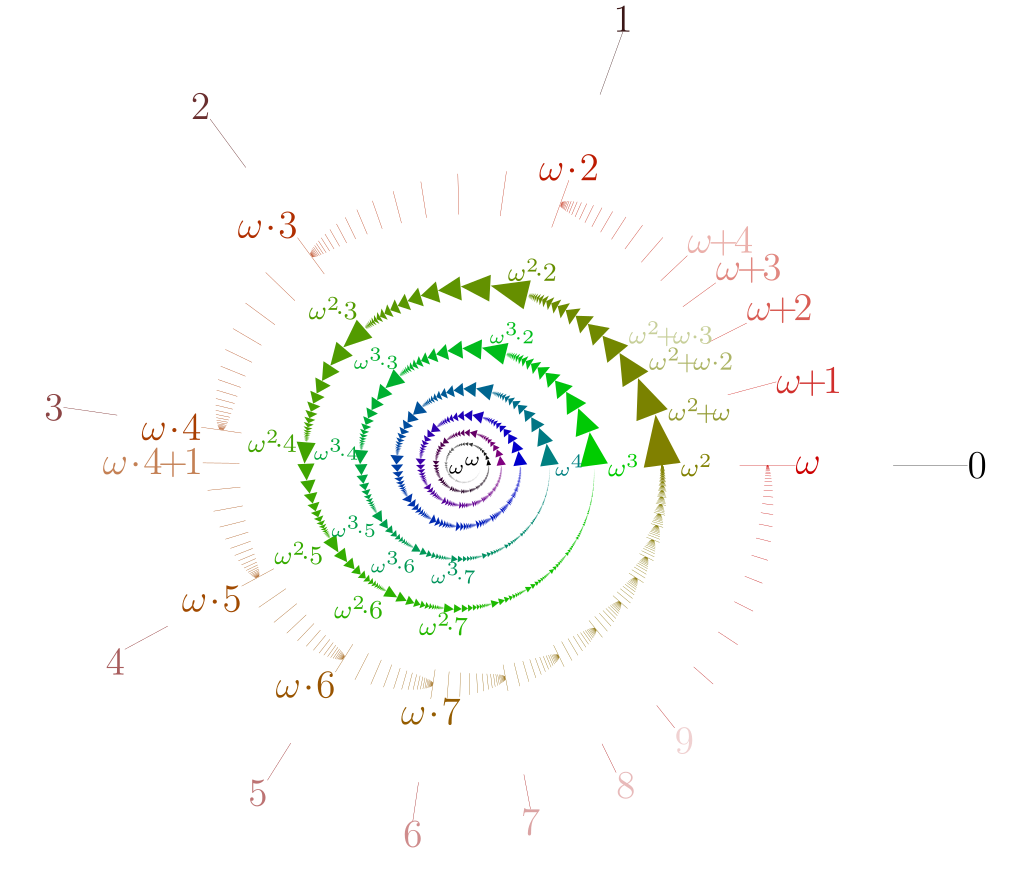
\includegraphics[scale=.49]{Omega_color.png}




%%%%%%%
\clearpage

\section{Ordinal Precedence v. Cardinal Precedence}

We have discussed two different precedence relations, $<_0$ and $<$:

\begin{itemize}
\item $<_o$ is the precedence relation for ordinals. 

$\alpha <_o \beta$ means that $\alpha$ precedes $\beta$ in the hierarchy of ordinals.

\item $<$ is an ordering of set-cardinality. 

$|A| < |B|$ means that there is an injection from $A$ to $B$ (but no bijection).

\end{itemize}

\fbox{\emph{Important:} $\alpha <_o \beta$ does not entail $|\alpha| < |\beta|$.}


\section{Ordinals as Blueprints for Large Sets}


\begin{itemize}
\item An ordinal can be used as a ``blueprint'' for a sequence of applications of the power set and union operations. 

\item The farther up an ordinal is in the hierarchy of ordinals, the longer the sequence, and the greater the cardinality of the end result.


\end{itemize}
Specifically, each ordinal $\alpha$ can be used to characterize the set $\mathfrak{B}_\alpha$:
\[
\mathfrak{B}_\alpha=
\begin{cases}
\mathbb{N}, \text{ if $\alpha = 0$}\\
\powerset(\mathfrak{B}_\beta), \text{ if $\alpha = \beta'$}\\
\bigcup \{\mathfrak{B}_\gamma : \gamma <_o \alpha\} \text{ if $\alpha$ is a limit ordinal (other than 0)}
\end{cases}
\]

\section{Later Ordinals, Bigger Cardinalities}

\begin{itemize}
\item By Cantor's Theorem: if $\alpha <_o \beta$, then $|\mathfrak{B}_\alpha| < |\mathfrak{B}_\beta|$.

\item For instance: 
$$\omega <_o (\omega \times \omega) <_o \omega^\omega <_o {^\omega\omega} \text{. So: } |\mathfrak{B}_{\omega}| < |\mathfrak{B}_{\omega \times \omega}| < |\mathfrak{B}_{\omega^\omega}| < |\mathfrak{B}_{^\omega\omega}|.$$

\end{itemize}


\section{Initial Ordinals}


\begin{itemize}

\item \textbf{Initial ordinal}: an ordinal that precedes all other ordinals of the same cardinality.

\item An initial ordinal $\kappa$ can be used as proxy or representative for its own cardinality

\item Abusing notation with `$\kappa$' as a cardinal, we let $\kappa = |\text{the ordinal called }`\kappa\text{'}|$
%JH: I think the following is a confusing or misleading statement: $\kappa = |\kappa|$.

\end{itemize}


\section{The Beth Hierarchy}


\begin{itemize}

\item $\beth_\alpha \text{ (read ``beth-alpha'') is the initial ordinal of cardinality } |\mathfrak{B}_\alpha|$.

\item So, abusing notation and letting `$\beth_\alpha$' now denote a cardinal, ``$\beth_\alpha = |\mathfrak{B}_\alpha|$''

%$\beth_\alpha$ is an ordinal of cardinality $|\mathfrak{B}_\alpha|$ and abusing notation, the cardinal ``$\beth_\alpha = |\mathfrak{B}_\alpha|$''

\item $\beth_0 = |\mathbb{N}|$ and $\beth_{0'} = |\powerset(\mathbb{N})|$ (so $\beth_{0'}$ is an \textbf{uncountable} ordinal). 


\end{itemize}
\vspace{2mm}
\noindent
Since the beths are \emph{ordinals}, they can be used to define sets bigger than anything we've considered so far. For instance: 

\begin{itemize}

\item $\mathfrak{B}_{\beth_{0'}}$ (where $\beth_{0'} = |\powerset(\mathbb{N})|$)

\item $\mathfrak{B}_{\beth_{\beth_\omega}}$ (where $\beth_{\beth_\omega} = |\mathfrak{B}_{\beth_{\omega}}|$)


\end{itemize}


\section{The Continuum Hypothesis}
\begin{description}
\item[Continuum Hypothesis] There is no set $A$ such that \(\beth_0 < |A| < \beth_1\). 
\item[Generalized CH] There is no set \(A\) such that \(\beth_\alpha < |A| < \beth_{\alpha + 1}\).
\end{description}





\com{
\section{The Aleph Hierarchy}


\begin{itemize}

\item \(\aleph_{\alpha}\) (read ``aleph-alpha'') is the first infinite ordinal of cardinality greater than every \(\aleph_\beta\) \((\beta <_o \alpha)\).

\item \(\aleph_{\alpha}\) is an initial ordinal. So \(\aleph_{\alpha} = |\aleph_{\alpha}|\).


\end{itemize}
\emph{Note:} The aleph-hierarchy includes \emph{every} infinite size.\footnote{Assuming the Axiom of Choice.}}


\section{The Burali-Forti Paradox}

Suppose, for \emph{reductio}, that $\Omega$ is the set of all ordinals. Then: 
\begin{itemize}

\item Since $\Omega$ consists of every ordinal, it consists of every ordinal that's been introduced so far. But a new ordinal is just the set of every ordinal that's been introduced so far. So: \textbf{$\Omega$  is an ordinal}.

\item If $\Omega$ was itself an ordinal, it would be a member of itself (and therefore have itself as a predecessor). But no ordinal can be its own predecessor. So: \textbf{$\Omega$  is not an ordinal}.

\end{itemize}
So there is no set of all ordinals!



\end{document}




